\documentclass[a4paper,12pt]{article}

\usepackage[top=2.5cm, bottom=2.5cm, left=3.175cm, right=3.175cm]{geometry}
\usepackage{polski}
\usepackage[utf8]{inputenc}
\usepackage{xcolor}
\usepackage{graphicx}
\usepackage{titlesec}
\usepackage{indentfirst}
\usepackage{amsmath}
\usepackage{float}
\usepackage{minted}
\usepackage[section]{placeins}

% \usetikzlibrary{positioning}

\graphicspath{{images/}}

\numberwithin{equation}{section}

\newminted{python}{breaklines,python3,linenos,frame=single}

\usepackage[pdftex,
            pdfauthor={Cezary Bober, Michał Kruczek},
            pdftitle={Dokumentacja projektu z przedmiotu Grafika Komputerowa},
            pdfsubject={Microcar Flex Furgon}]{hyperref}

\begin{document}

\pagenumbering{gobble}

\begin{titlepage}
    \includegraphics[height=1.75cm]{prz_pl.png}
    \hfill
    \includegraphics[height=1.75cm]{weii_pl.png}
    
    \centering
    \vfill
    
    {\Huge \textbf{Dokumentacja projektu z przedmiotu Grafika Komputerowa} \par}
	\vspace{1.5cm}
	{\LARGE Microcar Flex Furgon \par}
	
	\vfill
    
    {\Large \textbf{Cezary Bober} \par}
    {\Large \textbf{Michał Kruczek} \par}
    
    \vfill
    
    {\LARGE Rzeszów, 2019\par}
\end{titlepage}

\setlength{\parskip}{0.3cm}
\setlength{\parindent}{1cm}
\pagenumbering{arabic}
\setcounter{page}{2}

\tableofcontents
\pagebreak

\section{Opis projektu}

\section{Powstawanie projektu}
\subsection{Hello World}
\subsection{Utworzenie podłoża}

\subsection{Stworzenie modeli 3D}

\begin{figure}[H]
    \centering
    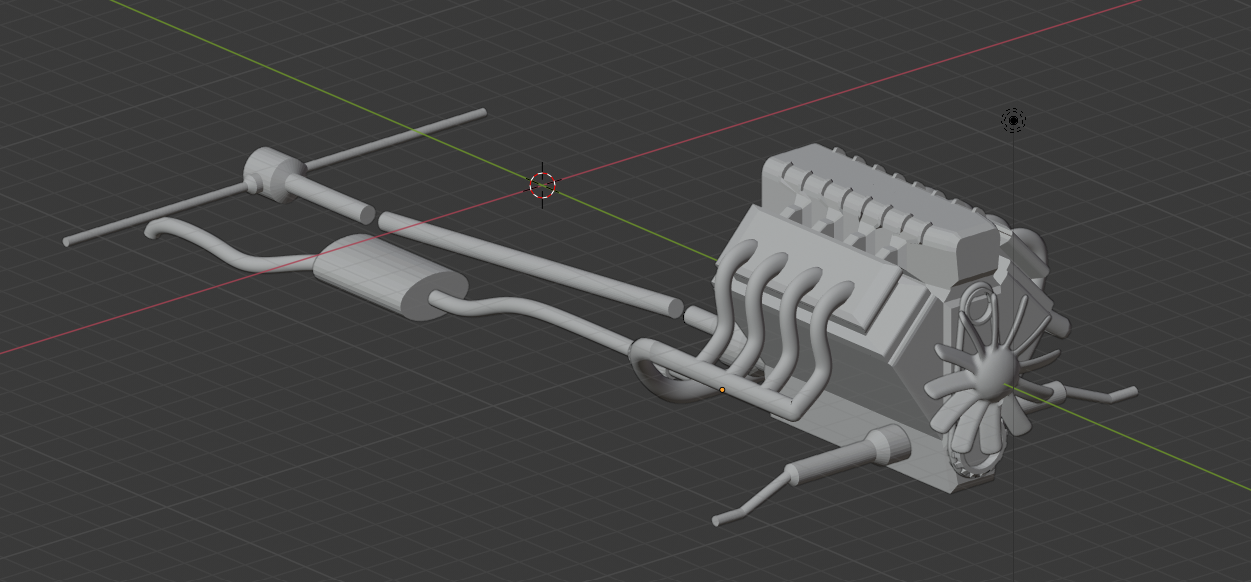
\includegraphics[width=\textwidth]{podwozie.png}
    \caption{Podwozie samochodu}
    \label{fig:podwozie}
    % \vspace{0.5cm}
\end{figure}


\subsection{Implementacja modeli w programie}
\subsection{Ożywienie samochodu}

\section{Podsumowanie}

% \begin{pythoncode}
% def forward(self, x):
%     y, sum_inputs = [x], []
%     for i in range(len(self.layers) + 1):
%         f = self.linear if i == len(self.layers) else self.activation
%         s = [np.dot(y[i], w) for w in self.weights[i]] + self.biases[i]
%         y.append(f(s))
%         sum_inputs.append(s)
%     return y, sum_inputs
% \end{pythoncode}


% \pagebreak
\begin{thebibliography}{9}
    \addcontentsline{toc}{section}{Literatura}
    \bibitem{zajdel_9} T. Gałaj, \emph{Learn OpenGL}, \href{https://shot511.github.io/pages/learnopengl/}{https://shot511.github.io/pages/learnopengl/}
\end{thebibliography}

\end{document}